\documentclass[tikz,border=1mm]{standalone}

\usepackage{ifthen}
\usepackage{fp} % 处理浮点数计算
\usetikzlibrary{calc}
% 初始化全局变量
\xdef\totalOffset{0}

% 定义网络层宏
\newcommand{\networkLayer}[9]{
    % 解析参数
    \def\hw{#1} % 层的高度和宽度
    \def\c{#2}  % 层的深度
    \def\x{#3}  % X 方向偏移量
    \def\y{#4}  % Y 方向偏移量
    \def\z{#5}  % Z 方向偏移量
    \def\inText{#7} % 层的标签
   

    % 如果 name 为 "start",则重置 totalOffset
    \ifthenelse{\equal{#8}{start}}{\xdef\totalOffset{0}}{}

    % 计算当前层的偏移量
    \FPeval{\currentOffset}{\totalOffset + \x} % 计算当前偏移量
    \FPeval{\newTotalOffset}{\currentOffset + \c} % 计算新的总偏移量
    \xdef\totalOffset{\newTotalOffset} % 更新总偏移量

    % 定义 3D 坐标
    \coordinate (#8_front) at  (\currentOffset+\c, \z, \y);
    \coordinate (#8_back) at   (\currentOffset, \z, \y);
    \coordinate (#8_top) at    (\currentOffset+\c/2, \z+\hw/2, \y);
    \coordinate (#8_bottom) at (\currentOffset+\c/2, \z-\hw/2, \y);

    % 定义立方体的角点
    \coordinate (blr) at (\c+\currentOffset,  -\hw/2+\z,  -\hw/2+\y);
    \coordinate (bur) at (\c+\currentOffset,   \hw/2+\z,  -\hw/2+\y);
    \coordinate (bul) at (0 +\currentOffset,   \hw/2+\z,  -\hw/2+\y);
    \coordinate (fll) at (0 +\currentOffset,  -\hw/2+\z,   \hw/2+\y);
    \coordinate (flr) at (\c+\currentOffset,  -\hw/2+\z,   \hw/2+\y);
    \coordinate (fur) at (\c+\currentOffset,   \hw/2+\z,   \hw/2+\y);
    \coordinate (ful) at (0 +\currentOffset,   \hw/2+\z,   \hw/2+\y);

    % 连接前一层
    \ifthenelse{\equal{#9}{}}{}{
        \foreach \val in #9 {
            \draw[line width=0.3mm] (\val) -- (#8_back);
        }
    }

    % 绘制立方体
    \draw[line width=0.3mm] (blr) -- (bur) -- (bul);
    \draw[line width=0.3mm] (fll) -- (flr) node[midway,below] {\inText} -- (fur) -- (ful) -- (fll);
    \draw[line width=0.3mm] (blr) -- (flr);
    \draw[line width=0.3mm] (bur) -- (fur);
    \draw[line width=0.3mm] (bul) -- (ful);

    \def\b{0.02}
    % 绘制前平面
	\filldraw[#6] ($(fll)+(\b,\b,0)$) -- ($(flr)+(-\b,\b,0)$) -- ($(fur)+(-\b,-\b,0)$) -- ($(ful)+(\b,-\b,0)$) -- ($(fll)+(\b,\b,0)$);
	\filldraw[#6] ($(ful)+(\b,0,-\b)$) -- ($(fur)+(-\b,0,-\b)$) -- ($(bur)+(-\b,0,\b)$) -- ($(bul)+(\b,0,\b)$);

	% 画上色的切片
	\ifthenelse {\equal{#6} {}}
	{} % 如果 #6 为空,则不绘制切片
	% 否则,绘制一个上色的切片
	{\filldraw[#6] ($(flr)+(0,\b,-\b)$) -- ($(blr)+(0,\b,\b)$) -- ($(bur)+(0,-\b,\b)$) -- ($(fur)+(0,-\b,-\b)$);}
}


\begin{document}

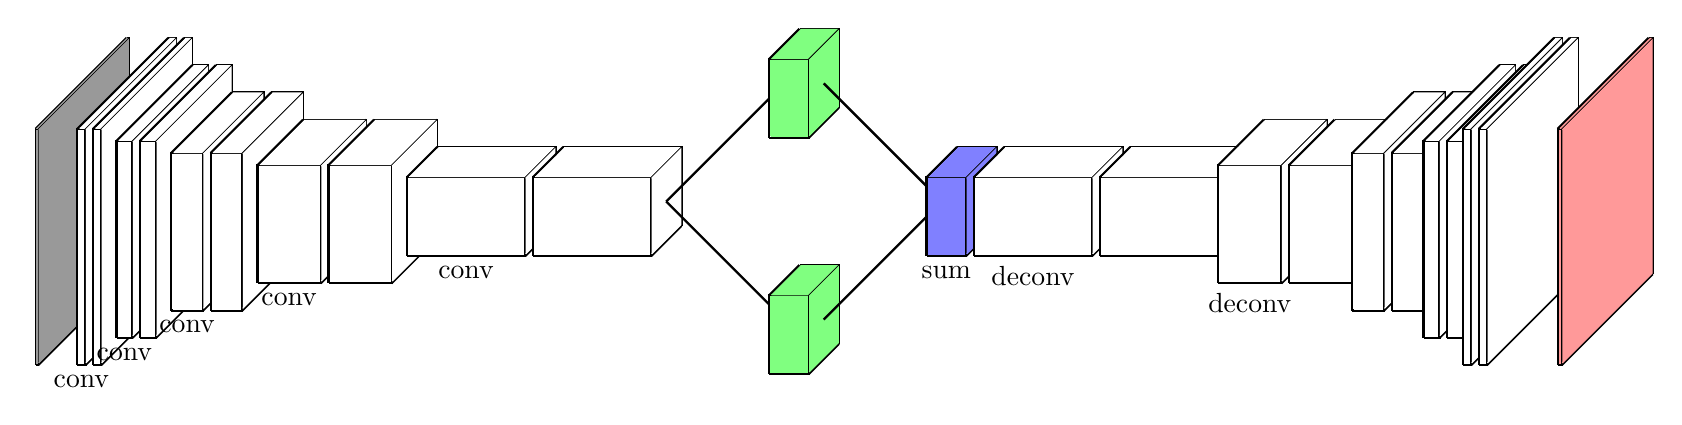
\begin{tikzpicture}

    % INPUT
    \networkLayer{3.0}{0.03}{0.0}{0.0}{0.0}{color=gray!80}{}{start}{}
    
    % ENCODER
    \networkLayer{3.0}{0.1}{0.5}{0.0}{0.0}{color=white}{conv}{}{}    % S1
    \networkLayer{3.0}{0.1}{0.1}{0.0}{0.0}{color=white}{}{}{}        % S2
    \networkLayer{2.5}{0.2}{0.1}{0.0}{0.0}{color=white}{conv}{}{}    % S1
    \networkLayer{2.5}{0.2}{0.1}{0.0}{0.0}{color=white}{}{}{}        % S2
    \networkLayer{2.0}{0.4}{0.1}{0.0}{0.0}{color=white}{conv}{}{}    % S1
    \networkLayer{2.0}{0.4}{0.1}{0.0}{0.0}{color=white}{}{}{}        % S2
    \networkLayer{1.5}{0.8}{0.1}{0.0}{0.0}{color=white}{conv}{}{}    % S1
    \networkLayer{1.5}{0.8}{0.1}{0.0}{0.0}{color=white}{}{}{}        % S2
    \networkLayer{1.0}{1.5}{0.1}{0.0}{0.0}{color=white}{conv}{}{}    % S1
    \networkLayer{1.0}{1.5}{0.1}{0.0}{0.0}{color=white}{}{mid}{}        % S2
    
    \networkLayer{1.0}{0.5}{1.5}{0.0}{-1.5}{color=green!50}{}{bot}{{mid_front}}
    \networkLayer{1.0}{0.5}{-0.5}{0.0}{1.5}{color=green!50}{}{top}{{mid_front}}
    \networkLayer{1.0}{0.5}{1.5}{0.0}{0.0}{color=blue!50}{sum}{}{{bot_front,top_front}}
    
    % DECODER
    \networkLayer{1.0}{1.5}{0.1}{0.0}{0.0}{color=white}{deconv}{}{} % S1
    \networkLayer{1.0}{1.5}{0.1}{0.0}{0.0}{color=white}{}{}{}       % S2
    \networkLayer{1.5}{0.8}{0.1}{0.0}{0.0}{color=white}{deconv}{}{} % S1
    \networkLayer{1.5}{0.8}{0.1}{0.0}{0.0}{color=white}{}{}{}       % S2
    \networkLayer{2.0}{0.4}{0.1}{0.0}{0.0}{color=white}{}{}{}       % S1
    \networkLayer{2.0}{0.4}{0.1}{0.0}{0.0}{color=white}{}{}{}       % S2
    \networkLayer{2.5}{0.2}{0.1}{0.0}{0.0}{color=white}{}{}{}       % S1
    \networkLayer{2.5}{0.2}{0.1}{0.0}{0.0}{color=white}{}{}{}       % S2
    \networkLayer{3.0}{0.1}{0.1}{0.0}{0.0}{color=white}{}{}{}       % S1
    \networkLayer{3.0}{0.1}{0.1}{0.0}{0.0}{color=white}{}{}{}       % S2
    
    % OUTPUT
    \networkLayer{3.0}{0.05}{0.9}{0.0}{0.0}{color=red!40}{}{}{}     % Pixelwise segmentation with classes.
    
    \end{tikzpicture}
    

\end{document}